\section{Конструкторская часть}

\subsection{Разработка нерекурсивного алгоритма нахождения расстояния Левенштейна}

Схема нерекурсивного алгоритма нахождения расстояния Левенштейна представлена на рисунке \ref{img:lev}.

\begin{figure}[h]
	\centering
	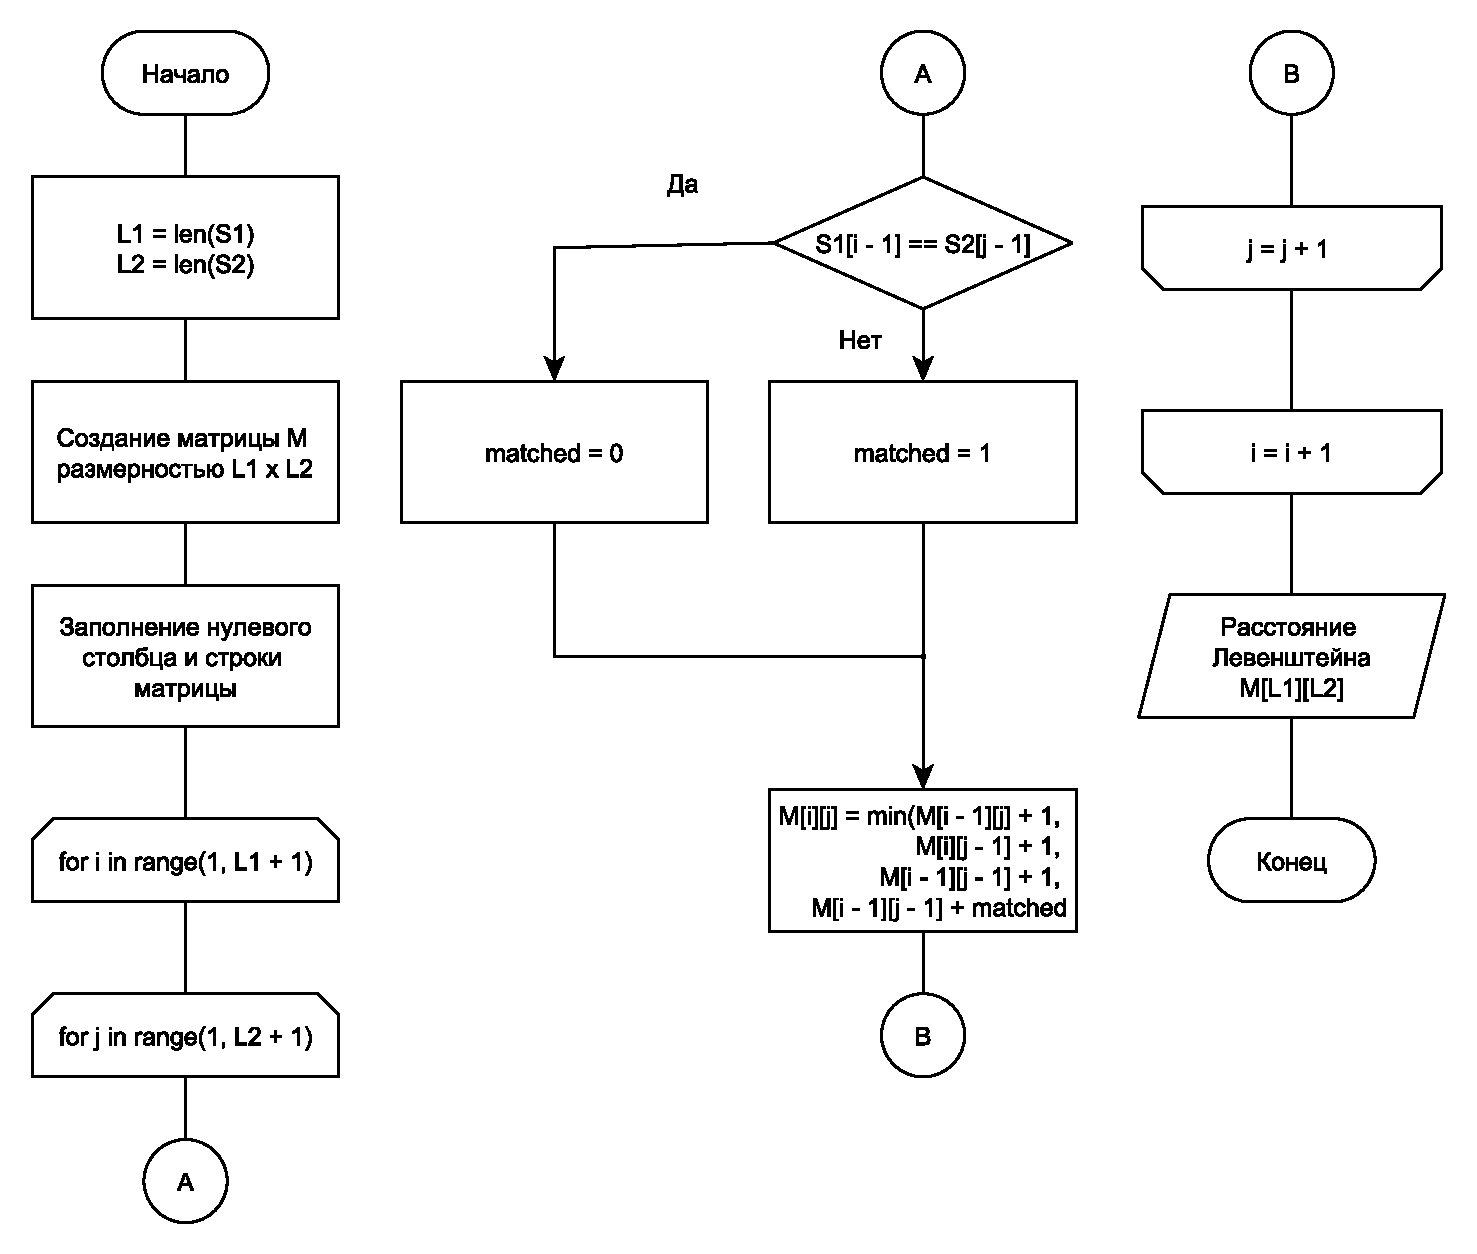
\includegraphics[scale=0.6]{images/lev.pdf}
	\caption{Схема нерекурсивного алгоритма нахождения расстояния Левенштейна}
	\label{img:lev}
\end{figure}

\newpage

\subsection{Разработка нерекурсивного алгоритма нахождения расстояния Дамерау-Левенштейна}

Схема нерекурсивного алгоритма нахождения расстояния Дамерау--Левенштейна представлена на рисунке \ref{img:dlev}.

\begin{figure}[h]
	\centering
	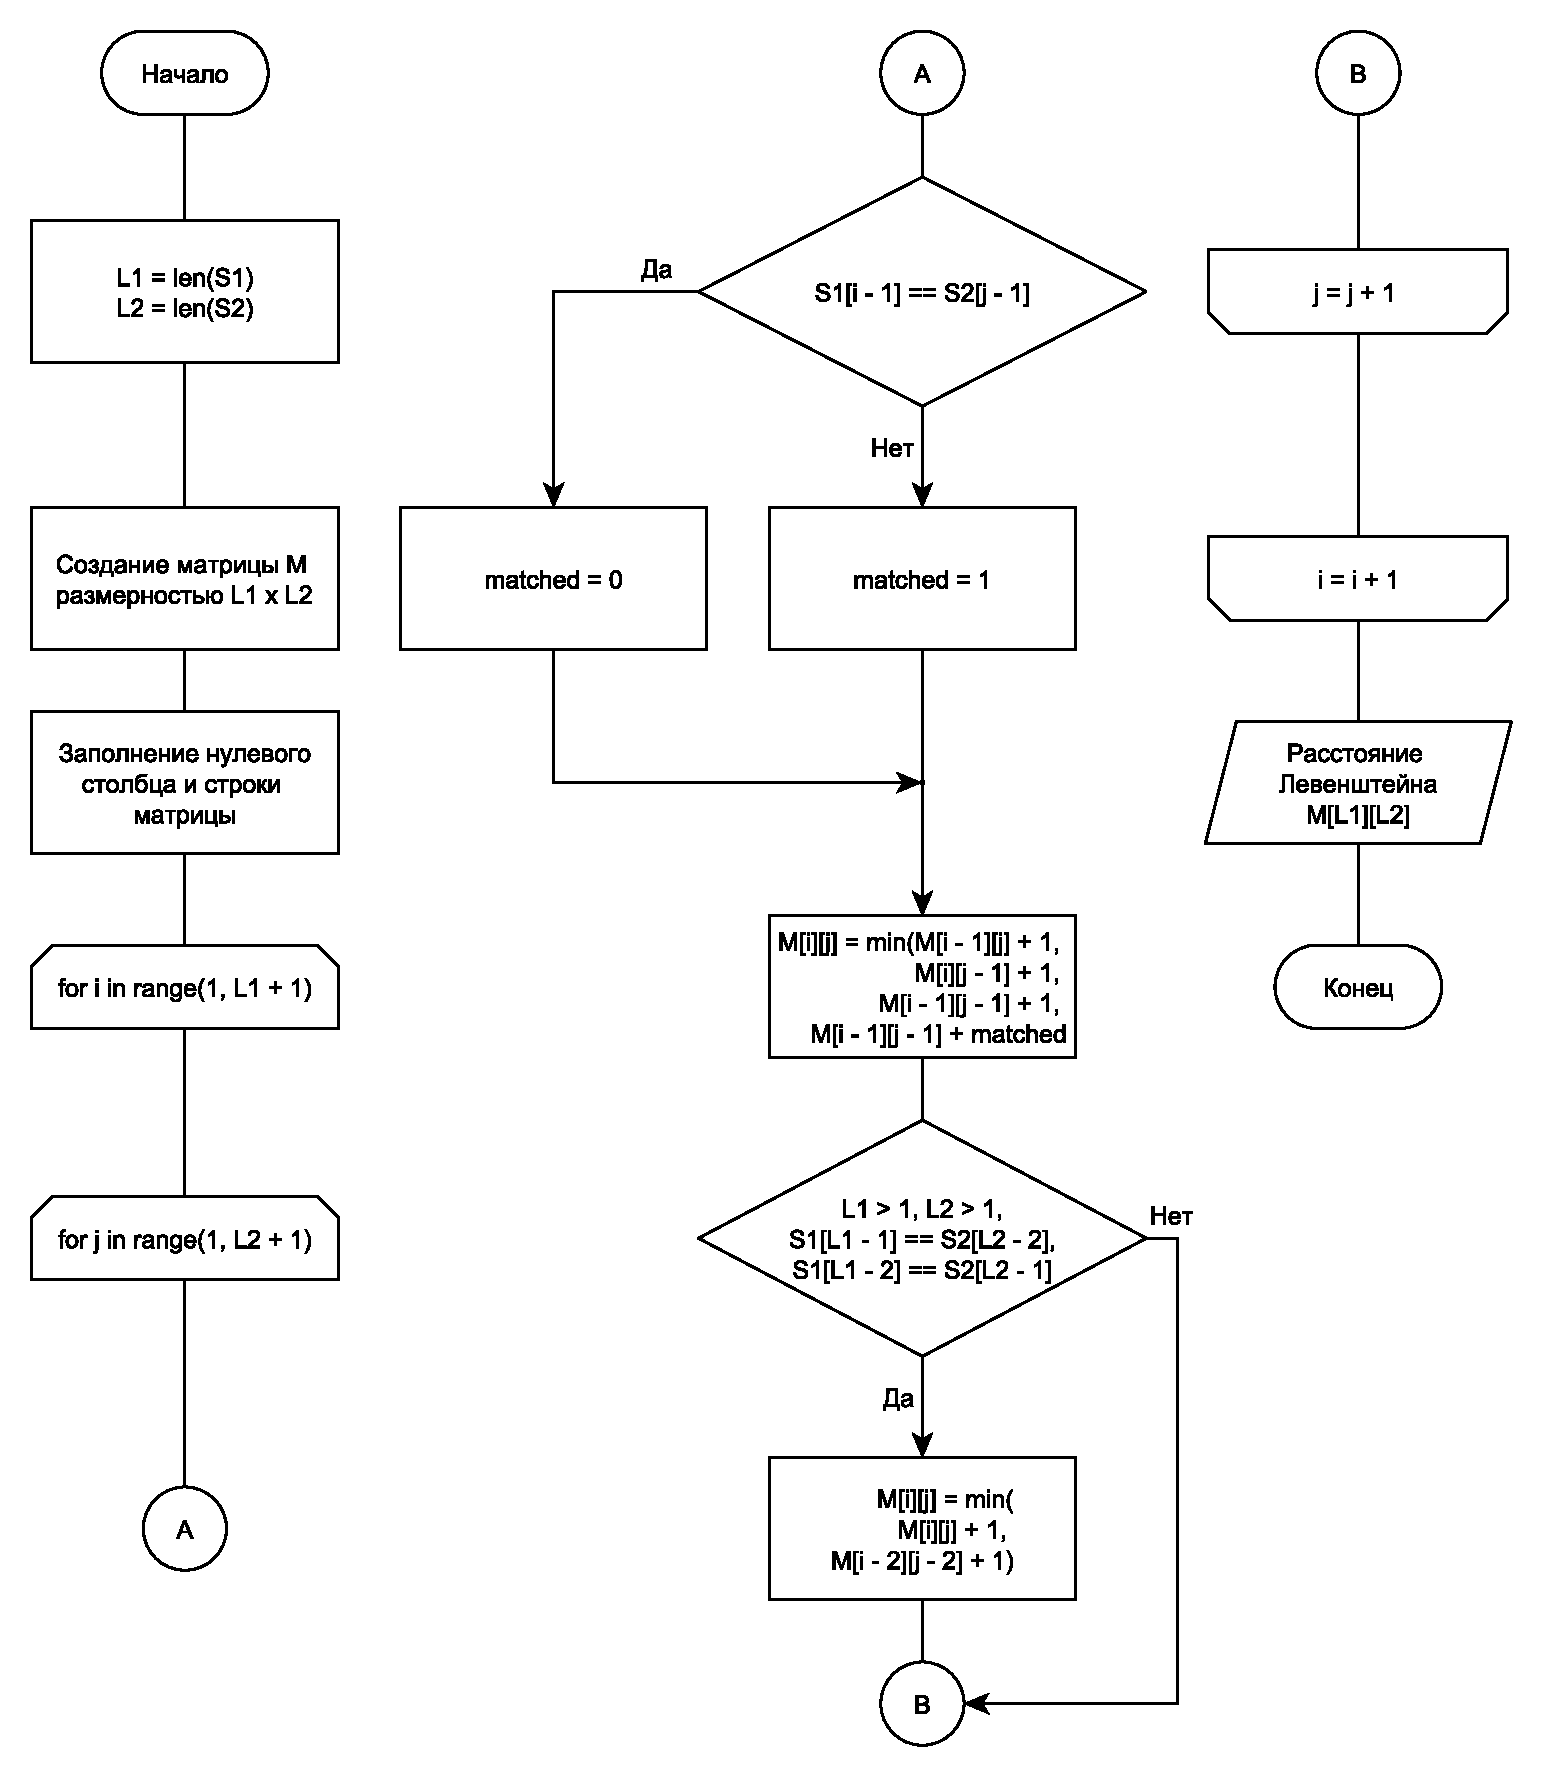
\includegraphics[scale=0.6]{images/dlev.pdf}
	\caption{Схема нерекурсивного алгоритма нахождения расстояния Дамерау-Левенштейна}
	\label{img:dlev}
\end{figure}


\subsection{Разработка рекурсивного алгоритма нахождения расстояния Дамерау-Левенштейна}

Схема рекурсивного алгоритма нахождения расстояния Дамерау--Левенштейна представлена на рисунке \ref{img:dlev_req}.

\begin{figure}[h]
	\centering
	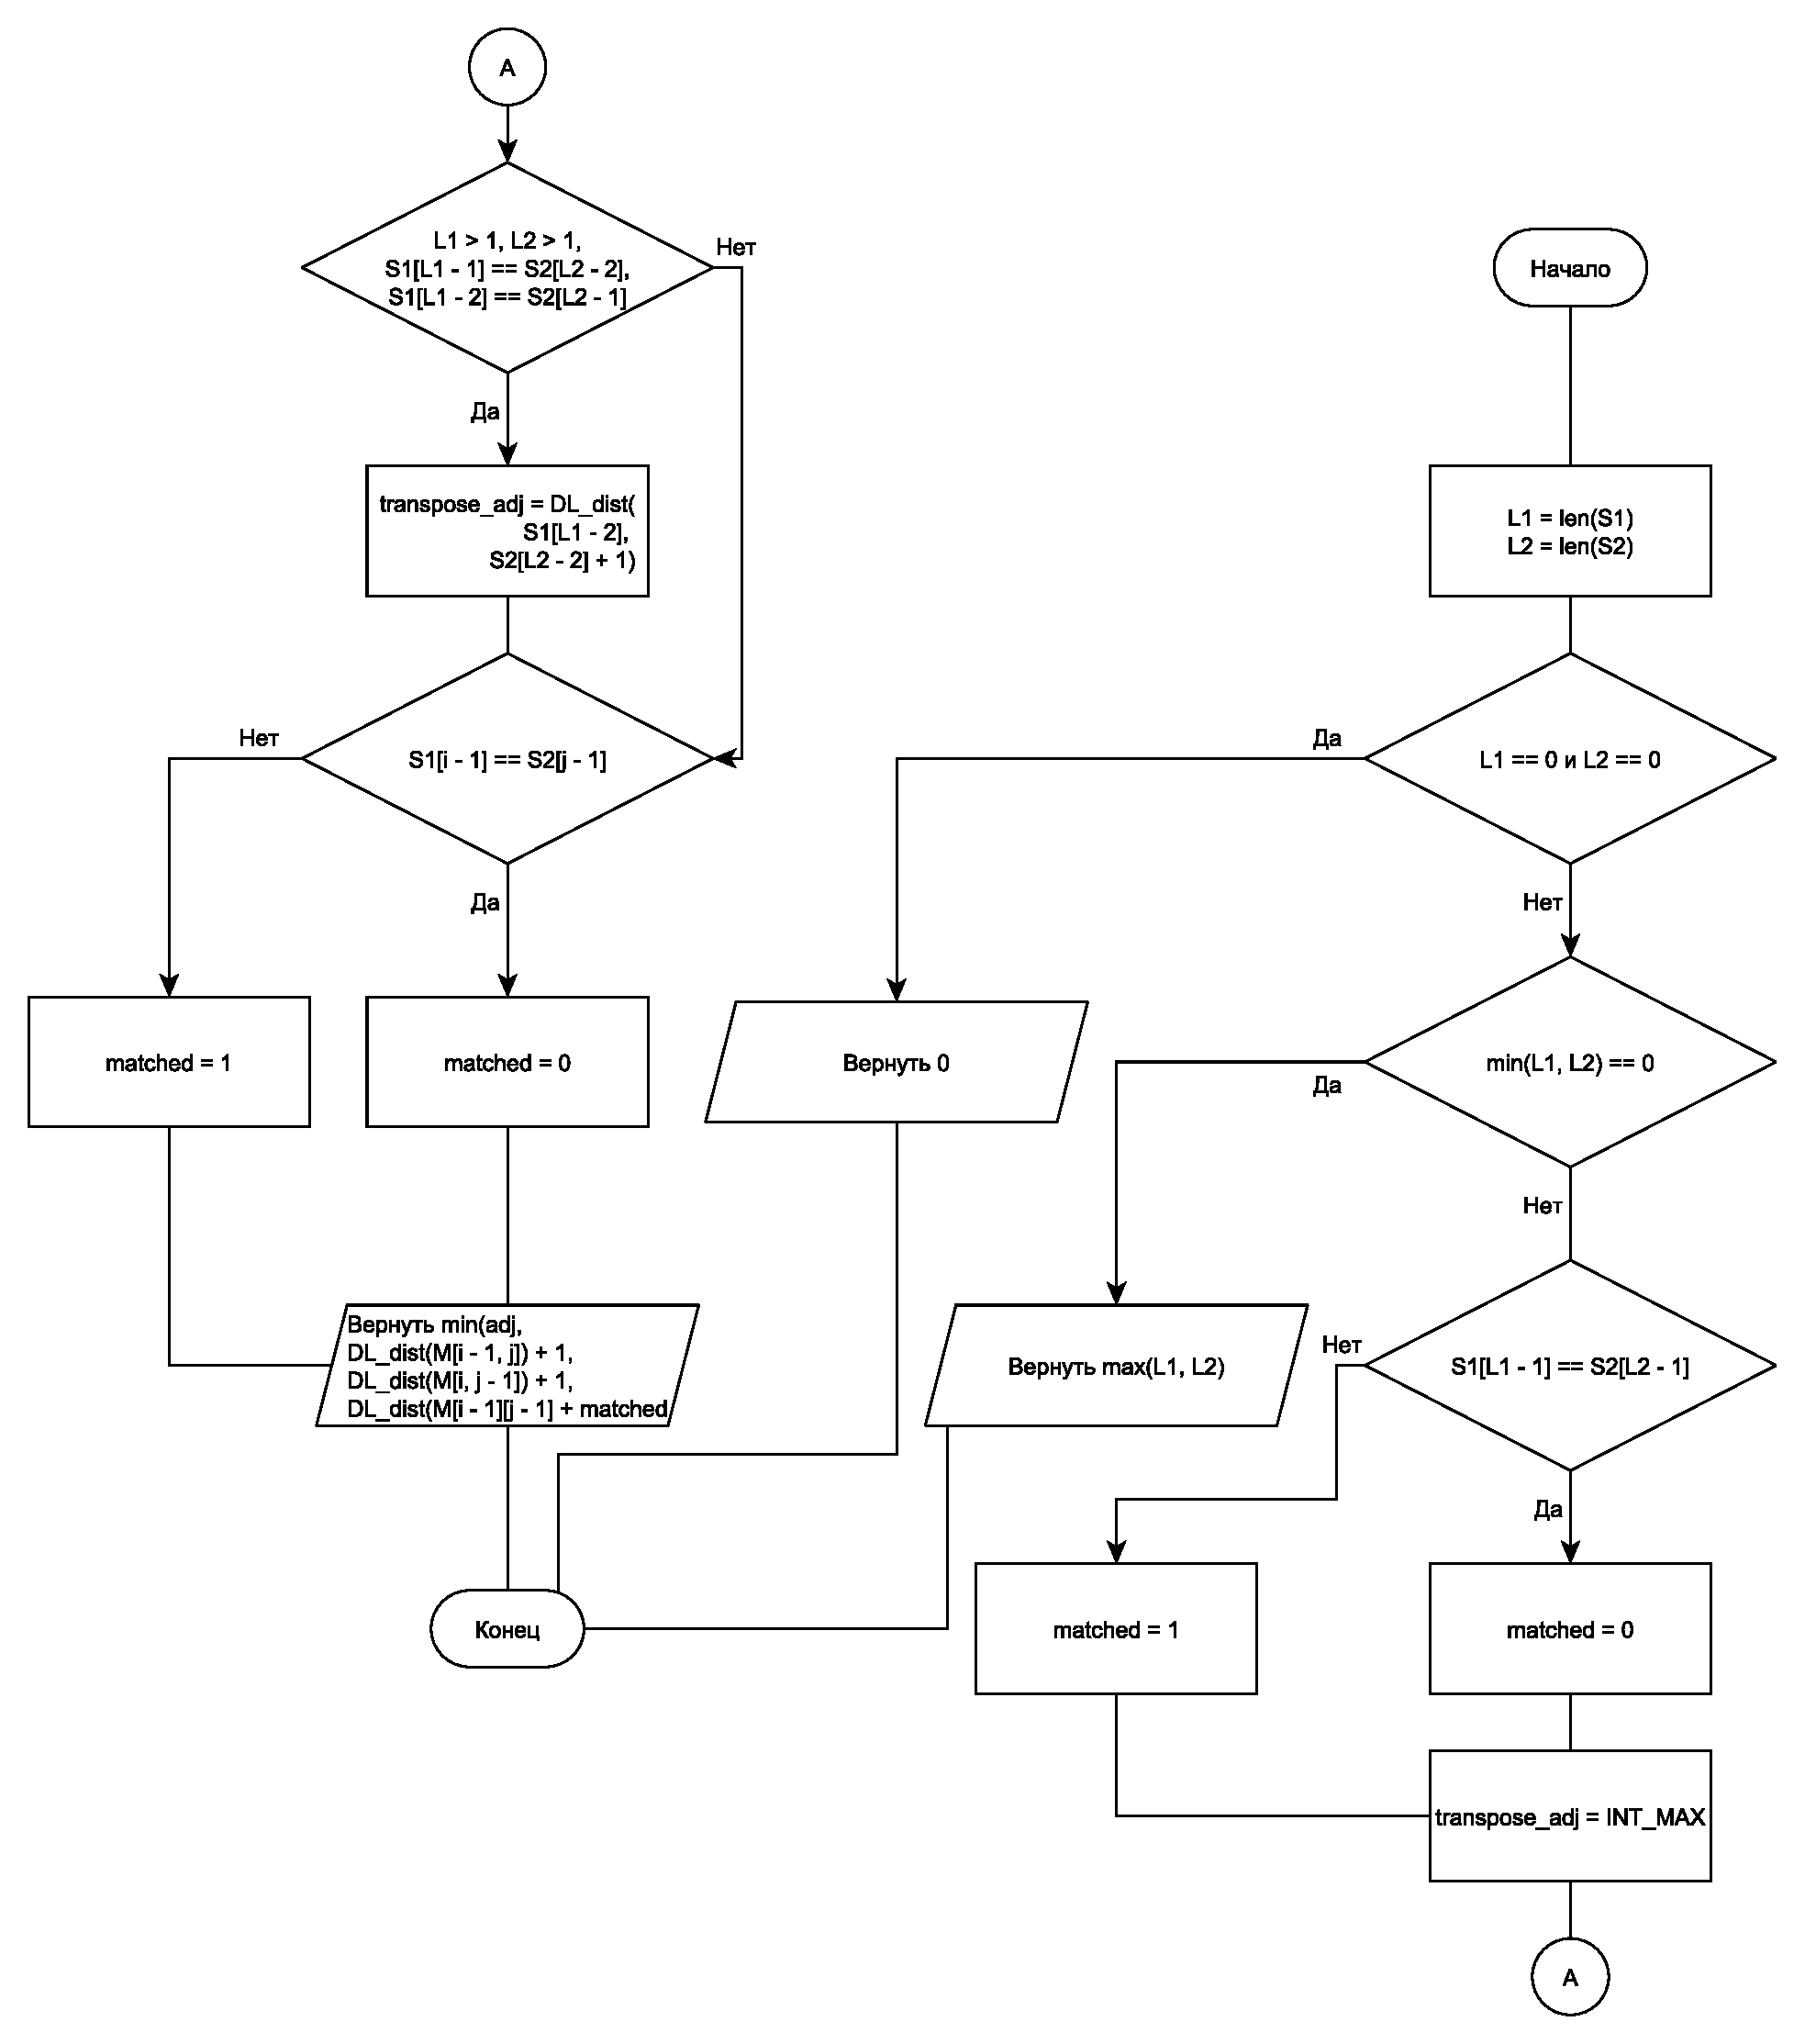
\includegraphics[scale=0.45]{images/dlev_req.pdf}
	\caption{Схема рекурсивного алгоритма нахождения расстояния Дамерау-Левенштейна}
	\label{img:dlev_req}
\end{figure}


\subsection{Разработка рекурсивного алгоритма нахождения расстояния Дамерау-Левенштейна с кэшем}

Схема рекурсивного алгоритма нахождения расстояния Дамерау--Левенштейна с кэшем представлена на рисунке \ref{img:dlev_req_cache}.

\begin{figure}[h]
	\centering
	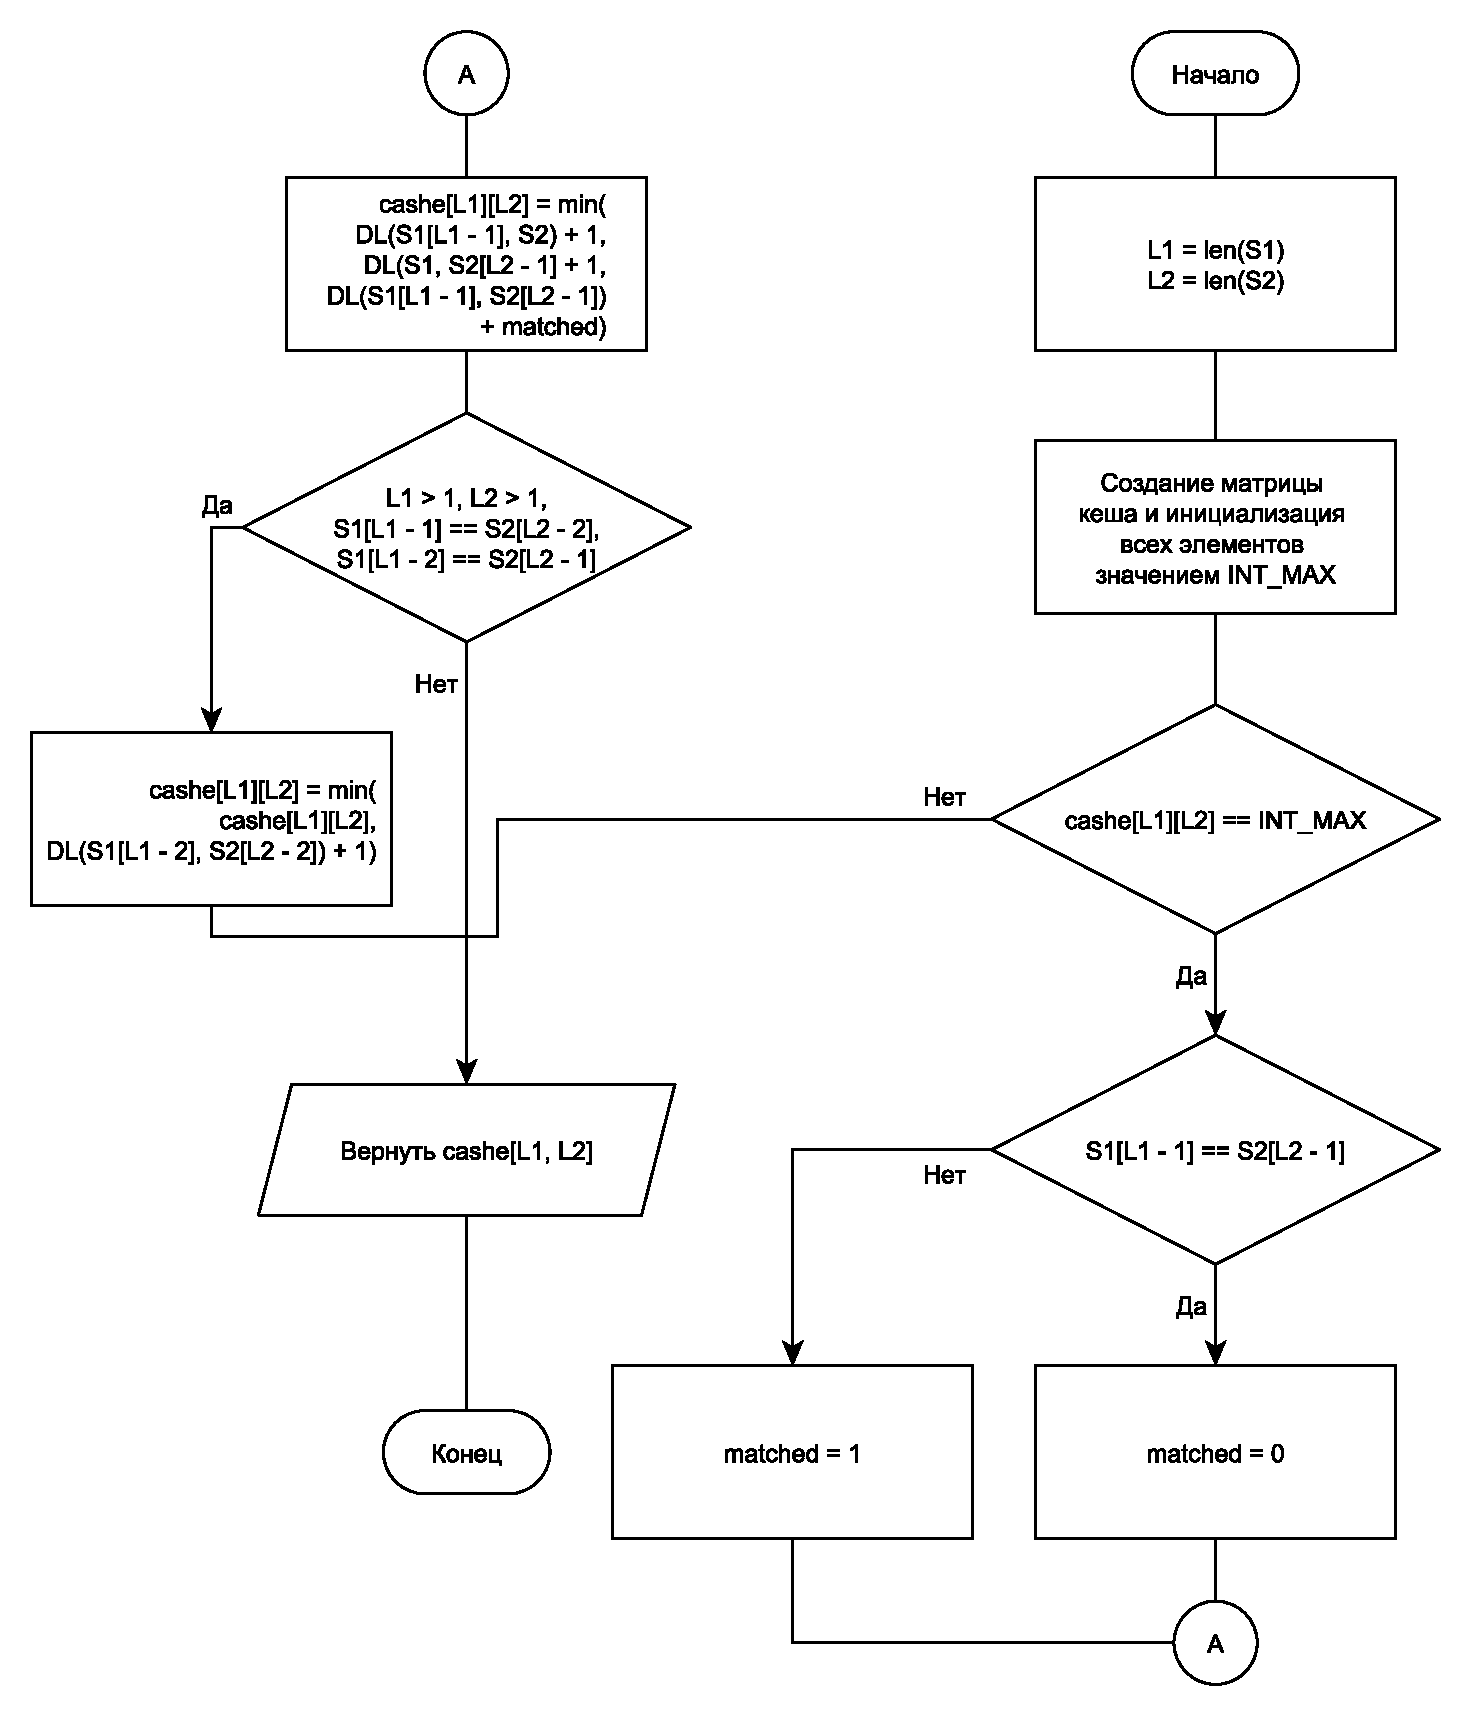
\includegraphics[scale=0.6]{images/dlev_req_cache.pdf}
	\caption{Схема рекурсивного алгоритма нахождения расстояния Дамерау-Левенштейна с кэшем}
	\label{img:dlev_req_cache}
\end{figure}

